\documentclass[11pt,a4paper,oneside]{book}
\usepackage[a4paper, portrait, margin=1.1in]{geometry}
% \documentclass[11pt,a4paper,twoside,openright]{book}
\usepackage{url}
\usepackage{makeidx}
\usepackage{listings}
\usepackage{graphicx}
\usepackage{fancyhdr}
\usepackage{fancyvrb}
\usepackage[usenames,dvipsnames]{color}


\definecolor{lightgray}{rgb}{.95,.95,.95}
\definecolor{darkgray}{rgb}{.4,.4,.4}
\definecolor{green}{rgb}{.2,.6,.0}
\definecolor{lightblue}{rgb}{.0,.5,.7}
\definecolor{purple}{rgb}{0.6, .1, 0.62}

\lstdefinelanguage{JavaScript}{
  keywords={typeof, new, true, false, catch, function, return, null, catch, switch, var, if, in, while, do, else, case, break, throw, for},
  keywordstyle=\color{blue}\bfseries,
  ndkeywords={exports, this, console},
  ndkeywordstyle=\color{lightblue}\bfseries,
  identifierstyle=\color{black},
  sensitive=false,
  comment=[l]{//},
  morecomment=[s]{/*}{*/},
  commentstyle=\color{green}\ttfamily,
  stringstyle=\color{purple}\ttfamily,
  morestring=[b]',
  morestring=[b]"
}

\lstdefinelanguage{Java}{
  keywords={typeof, new, true, false, catch, function, return, null, catch, switch, var, if, in, while, do, else, case, break, throw, String, Integer, int, Object, for, long, Runnable},
  keywordstyle=\color{blue}\bfseries,
  ndkeywords={import, this, class ,public, private, static, void, implements, extends},
  ndkeywordstyle=\color{lightblue}\bfseries,
  identifierstyle=\color{black},
  sensitive=false,
  comment=[l]{//},
  morecomment=[s]{/*}{*/},
  commentstyle=\color{green}\ttfamily,
  stringstyle=\color{purple}\ttfamily,
  morestring=[b]',
  morestring=[b]"
}

\lstdefinelanguage{KRE}{
  keywords={select, when, setting, with, http},
  keywordstyle=\color{blue}\bfseries,
  ndkeywords={rule},
  ndkeywordstyle=\color{lightblue}\bfseries,
  identifierstyle=\color{black},
  sensitive=false,
  morecomment=[s]{re\#}{\#},
  commentstyle=\color{green}\ttfamily,
  stringstyle=\color{purple}\ttfamily,
  morestring=[b]',
  morestring=[b]"
}

\lstdefinelanguage{OwnRule}{
  keywords={expression, event, condition, action, selector, symbol, instr, <, ==, >, >=, <=},
  keywordstyle=\color{blue}\bfseries,
  ndkeywords={on, if, do},
  ndkeywordstyle=\color{lightblue}\bfseries,
  identifierstyle=\color{black},
  sensitive=false,
  morecomment=[s]{re\#}{\#},
  commentstyle=\color{green}\ttfamily,
  stringstyle=\color{purple}\ttfamily,
  morestring=[b]',
  morestring=[b]"
}

% \lstdefinelanguage{JSON}{
%   identifierstyle=\color{black},
%   sensitive=false,
%   stringstyle=\color{purple}\ttfamily,
%   morestring=[b]',
%   morestring=[b]"
% }

% \definecolor{numb}{RGB}{150, 150, 150}
% \definecolor{delim}{RGB}{20,105,176}

% \lstdefinelanguage{JSON}{
%   identifierstyle=\color{black},
%   sensitive=false,
%   stringstyle=\color{purple}\ttfamily,
%   morestring=[b]',
%   morestring=[b]",
%     literate=
%      *{0}{{{\color{numb}0}}}{1}
%       {1}{{{\color{numb}1}}}{1}
%       {2}{{{\color{numb}2}}}{1}
%       {3}{{{\color{numb}3}}}{1}
%       {4}{{{\color{numb}4}}}{1}
%       {5}{{{\color{numb}5}}}{1}
%       {6}{{{\color{numb}6}}}{1}
%       {7}{{{\color{numb}7}}}{1}
%       {8}{{{\color{numb}8}}}{1}
%       {9}{{{\color{numb}9}}}{1}
%       % {\{}{{{\color{delim}{\{}}}}{1}
%       % {\}}{{{\color{delim}{\}}}}}{1}
%       % {[}{{{\color{delim}{[}}}}{1}
%       % {]}{{{\color{delim}{]}}}}{1}
% }

\lstdefinelanguage{RDF}{
  keywords={on, insert, if, do, delete, let, in},
  keywordstyle=\color{blue}\bfseries,
  % keywords=[2]{delta},
  % keywordstyle=[2]\color{green}\bfseries,
  ndkeywords={document, resource},
  ndkeywordstyle=\color{lightblue}\bfseries,
  identifierstyle=\color{black},
  sensitive=false,
  comment=[l]{//},
  morecomment=[s]{/*}{*/},
  commentstyle=\color{green}\ttfamily,
  stringstyle=\color{purple}\ttfamily,
  morestring=[b]',
  morestring=[b]"
}

\lstdefinelanguage{N3}{
  alsoletter=?,
  keywords={ ?x },
  keywordstyle=\color{blue}\bfseries,
  ndkeywords={exports, this},
  ndkeywordstyle=\color{lightblue}\bfseries,
  identifierstyle=\color{black},
  sensitive=false,
  comment=[l]{//},
  morecomment=[s]{/*}{*/},
  commentstyle=\color{green}\ttfamily,
  stringstyle=\color{purple}\ttfamily,
  morestring=[b]',
  morestring=[b]"
}

\lstdefinelanguage{XChange}{
  keywords={TRANSACTION, on, end, in, insert, from},
  keywordstyle=\color{blue}\bfseries,
  ndkeywords={xchange, var, resource},
  ndkeywordstyle=\color{lightblue}\bfseries,
  identifierstyle=\color{black},
  sensitive=false,
  comment=[l]{//},
  morecomment=[s]{/*}{*/},
  commentstyle=\color{green}\ttfamily,
  stringstyle=\color{purple}\ttfamily,
  morestring=[b]',
  morestring=[b]"
}

\lstset{
  language=JavaScript,
  % backgroundcolor=\color{lightgray},
  basicstyle=\footnotesize\ttfamily,
  extendedchars=true,
  frame=single,
  showstringspaces=false,
  showspaces=false,
  numbers=left,
  numberstyle=\tiny,
  numbersep=9pt,
  tabsize=2,
  breaklines=true,
  showtabs=false,
  captionpos=b,
  aboveskip=10pt,
  belowskip=10pt,
  xleftmargin=.3in
  % frameround=tttt,
  % boxpos=t
}


\makeatletter
\def\PY@reset{\let\PY@it=\relax \let\PY@bf=\relax%
    \let\PY@ul=\relax \let\PY@tc=\relax%
    \let\PY@bc=\relax \let\PY@ff=\relax}
\def\PY@tok#1{\csname PY@tok@#1\endcsname}
\def\PY@toks#1+{\ifx\relax#1\empty\else%
    \PY@tok{#1}\expandafter\PY@toks\fi}
\def\PY@do#1{\PY@bc{\PY@tc{\PY@ul{%
    \PY@it{\PY@bf{\PY@ff{#1}}}}}}}
\def\PY#1#2{\PY@reset\PY@toks#1+\relax+\PY@do{#2}}

\expandafter\def\csname PY@tok@gd\endcsname{\def\PY@tc##1{\textcolor[rgb]{0.63,0.00,0.00}{##1}}}
\expandafter\def\csname PY@tok@gu\endcsname{\let\PY@bf=\textbf\def\PY@tc##1{\textcolor[rgb]{0.50,0.00,0.50}{##1}}}
\expandafter\def\csname PY@tok@gt\endcsname{\def\PY@tc##1{\textcolor[rgb]{0.00,0.27,0.87}{##1}}}
\expandafter\def\csname PY@tok@gs\endcsname{\let\PY@bf=\textbf}
\expandafter\def\csname PY@tok@gr\endcsname{\def\PY@tc##1{\textcolor[rgb]{1.00,0.00,0.00}{##1}}}
\expandafter\def\csname PY@tok@cm\endcsname{\let\PY@it=\textit\def\PY@tc##1{\textcolor[rgb]{0.25,0.50,0.50}{##1}}}
\expandafter\def\csname PY@tok@vg\endcsname{\def\PY@tc##1{\textcolor[rgb]{0.10,0.09,0.49}{##1}}}
\expandafter\def\csname PY@tok@m\endcsname{\def\PY@tc##1{\textcolor[rgb]{0.40,0.40,0.40}{##1}}}
\expandafter\def\csname PY@tok@mh\endcsname{\def\PY@tc##1{\textcolor[rgb]{0.40,0.40,0.40}{##1}}}
\expandafter\def\csname PY@tok@go\endcsname{\def\PY@tc##1{\textcolor[rgb]{0.53,0.53,0.53}{##1}}}
\expandafter\def\csname PY@tok@ge\endcsname{\let\PY@it=\textit}
\expandafter\def\csname PY@tok@vc\endcsname{\def\PY@tc##1{\textcolor[rgb]{0.10,0.09,0.49}{##1}}}
\expandafter\def\csname PY@tok@il\endcsname{\def\PY@tc##1{\textcolor[rgb]{0.40,0.40,0.40}{##1}}}
\expandafter\def\csname PY@tok@cs\endcsname{\let\PY@it=\textit\def\PY@tc##1{\textcolor[rgb]{0.25,0.50,0.50}{##1}}}
\expandafter\def\csname PY@tok@cp\endcsname{\def\PY@tc##1{\textcolor[rgb]{0.74,0.48,0.00}{##1}}}
\expandafter\def\csname PY@tok@gi\endcsname{\def\PY@tc##1{\textcolor[rgb]{0.00,0.63,0.00}{##1}}}
\expandafter\def\csname PY@tok@gh\endcsname{\let\PY@bf=\textbf\def\PY@tc##1{\textcolor[rgb]{0.00,0.00,0.50}{##1}}}
\expandafter\def\csname PY@tok@ni\endcsname{\let\PY@bf=\textbf\def\PY@tc##1{\textcolor[rgb]{0.60,0.60,0.60}{##1}}}
\expandafter\def\csname PY@tok@nl\endcsname{\def\PY@tc##1{\textcolor[rgb]{0.63,0.63,0.00}{##1}}}
\expandafter\def\csname PY@tok@nn\endcsname{\let\PY@bf=\textbf\def\PY@tc##1{\textcolor[rgb]{0.00,0.00,1.00}{##1}}}
\expandafter\def\csname PY@tok@no\endcsname{\def\PY@tc##1{\textcolor[rgb]{0.53,0.00,0.00}{##1}}}
\expandafter\def\csname PY@tok@na\endcsname{\def\PY@tc##1{\textcolor[rgb]{0.49,0.56,0.16}{##1}}}
\expandafter\def\csname PY@tok@nb\endcsname{\def\PY@tc##1{\textcolor[rgb]{0.00,0.50,0.00}{##1}}}
\expandafter\def\csname PY@tok@nc\endcsname{\let\PY@bf=\textbf\def\PY@tc##1{\textcolor[rgb]{0.00,0.00,1.00}{##1}}}
\expandafter\def\csname PY@tok@nd\endcsname{\def\PY@tc##1{\textcolor[rgb]{0.67,0.13,1.00}{##1}}}
\expandafter\def\csname PY@tok@ne\endcsname{\let\PY@bf=\textbf\def\PY@tc##1{\textcolor[rgb]{0.82,0.25,0.23}{##1}}}
\expandafter\def\csname PY@tok@nf\endcsname{\def\PY@tc##1{\textcolor[rgb]{0.00,0.00,1.00}{##1}}}
\expandafter\def\csname PY@tok@si\endcsname{\let\PY@bf=\textbf\def\PY@tc##1{\textcolor[rgb]{0.73,0.40,0.53}{##1}}}
\expandafter\def\csname PY@tok@s2\endcsname{\def\PY@tc##1{\textcolor[rgb]{0.73,0.13,0.13}{##1}}}
\expandafter\def\csname PY@tok@vi\endcsname{\def\PY@tc##1{\textcolor[rgb]{0.10,0.09,0.49}{##1}}}
\expandafter\def\csname PY@tok@nt\endcsname{\let\PY@bf=\textbf\def\PY@tc##1{\textcolor[rgb]{0.00,0.50,0.00}{##1}}}
\expandafter\def\csname PY@tok@nv\endcsname{\def\PY@tc##1{\textcolor[rgb]{0.10,0.09,0.49}{##1}}}
\expandafter\def\csname PY@tok@s1\endcsname{\def\PY@tc##1{\textcolor[rgb]{0.73,0.13,0.13}{##1}}}
\expandafter\def\csname PY@tok@sh\endcsname{\def\PY@tc##1{\textcolor[rgb]{0.73,0.13,0.13}{##1}}}
\expandafter\def\csname PY@tok@sc\endcsname{\def\PY@tc##1{\textcolor[rgb]{0.73,0.13,0.13}{##1}}}
\expandafter\def\csname PY@tok@sx\endcsname{\def\PY@tc##1{\textcolor[rgb]{0.00,0.50,0.00}{##1}}}
\expandafter\def\csname PY@tok@bp\endcsname{\def\PY@tc##1{\textcolor[rgb]{0.00,0.50,0.00}{##1}}}
\expandafter\def\csname PY@tok@c1\endcsname{\let\PY@it=\textit\def\PY@tc##1{\textcolor[rgb]{0.25,0.50,0.50}{##1}}}
\expandafter\def\csname PY@tok@kc\endcsname{\let\PY@bf=\textbf\def\PY@tc##1{\textcolor[rgb]{0.00,0.50,0.00}{##1}}}
\expandafter\def\csname PY@tok@c\endcsname{\let\PY@it=\textit\def\PY@tc##1{\textcolor[rgb]{0.25,0.50,0.50}{##1}}}
\expandafter\def\csname PY@tok@mf\endcsname{\def\PY@tc##1{\textcolor[rgb]{0.40,0.40,0.40}{##1}}}
%\expandafter\def\csname PY@tok@err\endcsname{\def\PY@bc##1{\setlength{\fboxsep}{0pt}\fcolorbox[rgb]{1.00,0.00,0.00}{1,1,1}{\strut ##1}}}
\expandafter\def\csname PY@tok@kd\endcsname{\let\PY@bf=\textbf\def\PY@tc##1{\textcolor[rgb]{0.00,0.50,0.00}{##1}}}
\expandafter\def\csname PY@tok@ss\endcsname{\def\PY@tc##1{\textcolor[rgb]{0.10,0.09,0.49}{##1}}}
\expandafter\def\csname PY@tok@sr\endcsname{\def\PY@tc##1{\textcolor[rgb]{0.73,0.40,0.53}{##1}}}
\expandafter\def\csname PY@tok@mo\endcsname{\def\PY@tc##1{\textcolor[rgb]{0.40,0.40,0.40}{##1}}}
\expandafter\def\csname PY@tok@kn\endcsname{\let\PY@bf=\textbf\def\PY@tc##1{\textcolor[rgb]{0.00,0.50,0.00}{##1}}}
\expandafter\def\csname PY@tok@mi\endcsname{\def\PY@tc##1{\textcolor[rgb]{0.40,0.40,0.40}{##1}}}
\expandafter\def\csname PY@tok@gp\endcsname{\let\PY@bf=\textbf\def\PY@tc##1{\textcolor[rgb]{0.00,0.00,0.50}{##1}}}
\expandafter\def\csname PY@tok@o\endcsname{\def\PY@tc##1{\textcolor[rgb]{0.40,0.40,0.40}{##1}}}
\expandafter\def\csname PY@tok@kr\endcsname{\let\PY@bf=\textbf\def\PY@tc##1{\textcolor[rgb]{0.00,0.50,0.00}{##1}}}
\expandafter\def\csname PY@tok@s\endcsname{\def\PY@tc##1{\textcolor[rgb]{0.73,0.13,0.13}{##1}}}
\expandafter\def\csname PY@tok@kp\endcsname{\def\PY@tc##1{\textcolor[rgb]{0.00,0.50,0.00}{##1}}}
\expandafter\def\csname PY@tok@w\endcsname{\def\PY@tc##1{\textcolor[rgb]{0.73,0.73,0.73}{##1}}}
\expandafter\def\csname PY@tok@kt\endcsname{\def\PY@tc##1{\textcolor[rgb]{0.69,0.00,0.25}{##1}}}
\expandafter\def\csname PY@tok@ow\endcsname{\let\PY@bf=\textbf\def\PY@tc##1{\textcolor[rgb]{0.67,0.13,1.00}{##1}}}
\expandafter\def\csname PY@tok@sb\endcsname{\def\PY@tc##1{\textcolor[rgb]{0.73,0.13,0.13}{##1}}}
\expandafter\def\csname PY@tok@k\endcsname{\let\PY@bf=\textbf\def\PY@tc##1{\textcolor[rgb]{0.00,0.50,0.00}{##1}}}
\expandafter\def\csname PY@tok@se\endcsname{\let\PY@bf=\textbf\def\PY@tc##1{\textcolor[rgb]{0.73,0.40,0.13}{##1}}}
\expandafter\def\csname PY@tok@sd\endcsname{\let\PY@it=\textit\def\PY@tc##1{\textcolor[rgb]{0.73,0.13,0.13}{##1}}}
%\expandafter\def\csname PY@tok@err\endcsname{}

\def\PYZbs{\char`\\}
\def\PYZus{\char`\_}
\def\PYZob{\char`\{}
\def\PYZcb{\char`\}}
\def\PYZca{\char`\^}
\def\PYZam{\char`\&}
\def\PYZlt{\char`\<}
\def\PYZgt{\char`\>}
\def\PYZsh{\char`\#}
\def\PYZpc{\char`\%}
\def\PYZdl{\char`\$}
\def\PYZhy{\char`\-}
\def\PYZsq{\char`\'}
\def\PYZdq{\char`\"}
\def\PYZti{\char`\~}
% for compatibility with earlier versions
\def\PYZat{@}
\def\PYZlb{[}
\def\PYZrb{]}
\makeatother

% How deep numbering is applied to titles
\setcounter{secnumdepth}{3}
% \setcounter{tocdepth}{3}

% Prepare the word index
\makeindex

% Prepare header and footer
\pagestyle{fancy}
\fancyhf{}
\rhead{\footnotesize\leftmark}
\lfoot{Towards the Reactive Web}
\rfoot{\thepage}
\renewcommand{\headrulewidth}{0.3pt}
\renewcommand{\footrulewidth}{0.3pt}

% Apply page style also to chapter's first page
\makeatletter
\renewcommand\chapter{\if@openright\cleardoublepage\else\clearpage\fi
  \thispagestyle{fancy}%
  \global\@topnum\z@
  \@afterindentfalse
  \secdef\@chapter\@schapter}
\makeatother


\begin{document}

\frontmatter
	\begin{titlepage}
\begin{center}

% \title{\huge \textbf{Towards The Reactive Web}\vspace*{15 mm}}
% %\subtitle{Master Thesis Report}
% \date{\today}
% %\date{}
% %\author{Dominic Bosch \\ Departement Mathematics and Computer Science \\ University of Basel}
% \author{\fontsize{11}{9}\selectfont
% Master Thesis\\
% \vspace*{10 mm}\\
% Dominic Bosch\\
% Departement Mathematics and Computer Science\\
% University of Basel
% }
% \maketitle

\vspace*{4cm}
\HRule \\[0.4cm]
{ \huge \bfseries Towards Reactive Information Systems \\ and their Services \\[0.4cm] }
% { \huge \bfseries Towards The Reactive Web \\[0.4cm] }
\HRule \\[1.5cm]

% \textsc{\Large Departement Mathematics and Computer Science}\\[0.5cm]

\vspace*{.5cm}
\textit{\textsc{\LARGE Master Thesis}}\\
\vspace*{2.5cm}

% Author and supervisor
\begin{minipage}{0.4\textwidth}
\begin{flushleft} \large
\emph{Author:}\\
Dominic \textsc{Bosch}
\end{flushleft}
\end{minipage}
\begin{minipage}{0.4\textwidth}
\begin{flushright} \large
\emph{Supervisors:} \\
Prof. Dr.~Helmar \textsc{Burkhart}\\
Dr.~Martin \textsc{Guggisberg}
\end{flushright}
\end{minipage}

\vfill

% Bottom of the page
{\large \today} \\[1.5cm]
% {\large May 15, 2014} \\[1.5cm]



% \textsc{\LARGE University of Basel}\\

\includegraphics[width=0.15\textwidth]{figures/unilogoschwarz}%~\\[1cm]
\end{center}
\end{titlepage}

	\chapter*{Acknowledgment}
I would like to express my deep gratitude to my master thesis advisor, Prof. Dr. Helmar Burkhart, for his patience and constant encouragement to keep going further.
I also want to thank Dr. Martin Guggisberg for his very helpful advices and hints to existing technologies.
Besides my advisors, I would like to thank the members of the research group: Danilo Guerrera,
Antonio Maffia, Alexander Gr\"oflin and Robert Frank for their help, many interesting discussions and inputs.

I would like to thank my parents Silvia and Peter Bosch for their love, patience and financial support on my journey.
Special thanks go to my sister Svenja, her husband Andreas and their seven months old son Nico, who all kept me going with their joyfulness and irresistble smiles.
Finally I would like to thank my partner Kathrina Hagnauer for her patience and endless love.
	\tableofcontents

\mainmatter
	\chapter{Introduction}
The fast evolving web provides ever more data and functionalities, both in terms of volume and also complexity.
Together with the ubiquitous access to the web through mobile devices and their push notifications, users get flooded with informations and, in turn, also produce increasingly more information.
Governing the web's information flood is getting more difficult and even fairly impossible for human beings with the tools given.


It becomes important to the individual to be able to filter out personally important bits and pieces.
Basic filters are often available but they do not allow smart filtering in any way.
Also, apart from smart filtering of information, people should have the possibility to aggregate important information in their desired place and in a way it's most useful for themselves.
Such an aggregation implies access to services that consume data and produce an output, be it an answer or storing the data.
This means the user should get access to data and functionality services in a way that she can combine the possibilities in a suitable way to generated the most valuable output for her.
Even if the web service access gets simpler these days, the average user is not able to weild them.
The challenge to provide users with ways to handle these already simpler accessible services, called Web API's has received a notable amount of attention over the last few years.
% TODO
% It is a promising research field that leads towards reactivity in the web through programmability.


% % TODO Reactivity!! allgemein
% \index{Reactivity}

% % TODO Programmability of the Web
% \index{Programmability}



Currently only few possibilities exist in the web to turn the web into reactive entity, which allows to process information as it arises.

	
\chapter{Conceptual Model for Reactive Web Systems}
% NOTES / TODOs:
%
% Rahmenbedingungen
% Vorzuege
% Notwendigkeiten
% Architektur


\section{Event Condition Action (ECA) Model in the Web}
% NOTES / TODOs:
%
% Model / Schema
% Zeit / Verteiltheit
% RL <-> ECA
% why are we now suddenly responsive? we loosened up certain things

Existing ECA systems (List examples) all act on local data.
Looking at (Wikipedia...) their definition is actions on local data.
This does only add reactivity to these systems and not to the Web per se.

Such systems are merely event sinks which add fairly any value to the Web, except for the individual users and the system itself.
We are taking a step further and allow not only the chaining up of several remote ECA engines, but also the invocation of actions on any arbitrary Web accessible service.


\newpage
wow
	
\chapter{The "XYZ" Prototype System}

% NOTES / TODOs:
%
% Architecture scheme, implementation
% callback functions, hot plugin
% js-select selectors
% List of condition operators
% Why JS, why wasnt it used before? is it used now?
% Transactions in businesses, find use case. how would we lose events?
% Terminierungsproblem (compiler bau), loesungsansaetze



\section{Event Triggers}

Event Gathering is the E in ECA and without one of these letters such a system would not run.
It is of utmost importance to find as much as possible ways to get data into a system.



\subsection{Polling for Events}



\subsection{Webhooks}
Which 



\section{Actions}



\section{ECA Rules}



\section{Architecture}



\section{Asynchronous Systems \& Closures}
% NOTES / TODOs:
%
% Variable bindings
% Closures (https://developer.mozilla.org/en-US/docs/Web/JavaScript/Guide/Closures)$
% Closures are functions that refer to independent (free) variables. 
% In other words, the function defined in the closure 'remembers' the environment in which it was created in.

% write about arallel as well?

Often optimization approaches and programming language concepts require special attention to avoid common pitfalls.
When closures are used in asynchronous systems, developers need to be very careful not to end up with randomly inconsistent states.


Looking at an example of sequential code execution in figure~\ref{fig:Closures_Synchronous}, we see that function execution of \texttt{fA} is halted until function \texttt{fB} is finished.
If \texttt{fB} happens to be a latency-driven I/O operation the completion of \texttt{fA} could be deferred for a relatively long time.
While the application waits for the completion of the I/O operation, some remaining operations in \texttt{fA} could eventually already be executed without causing any race conditions.
\begin{figure}[h!]
\centering
  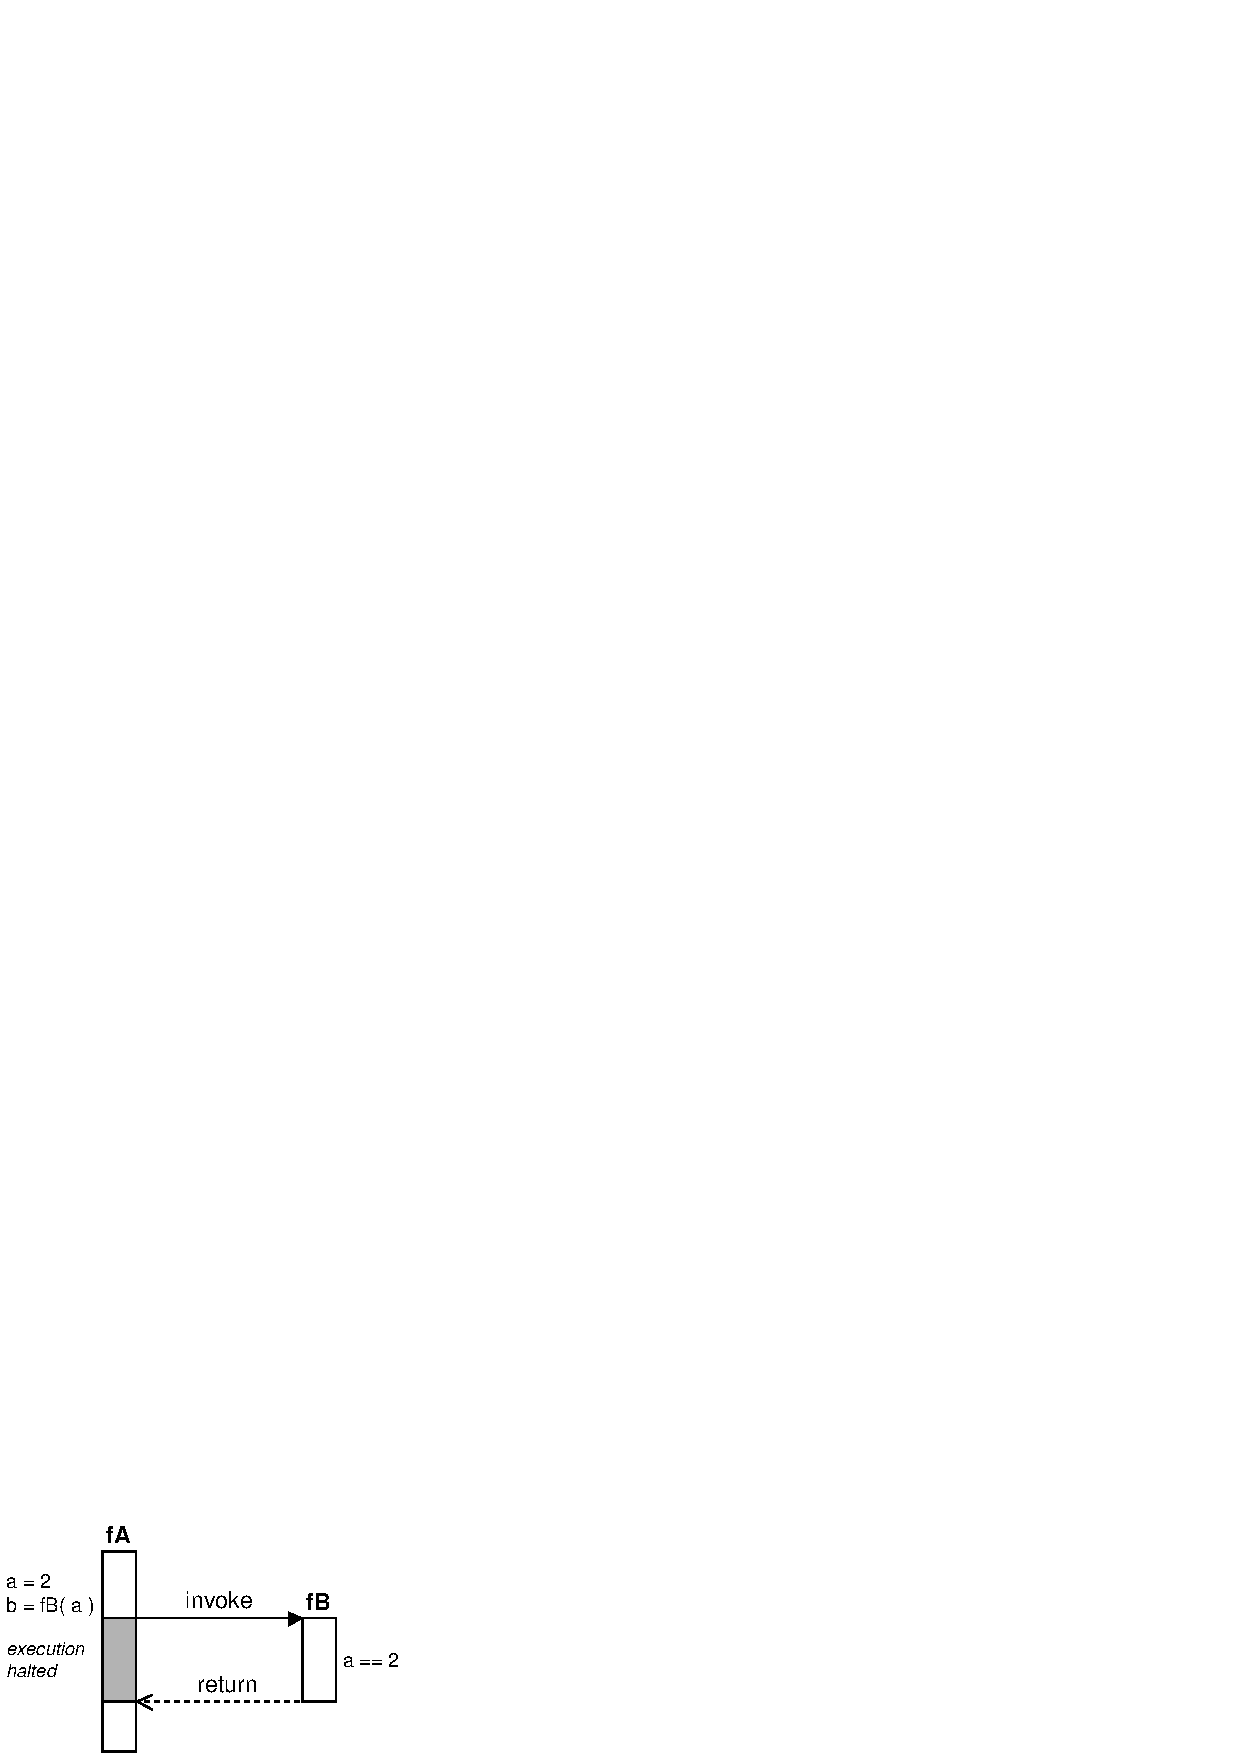
\includegraphics{figures/Closures_Synchronous}
\caption{Synchronous Function Call}
\label{fig:Closures_Synchronous}
\end{figure}


Asynchronous code execution, as shown in figure~\ref{fig:Closures_Asynchronous}, allows non-blocking and thus scalable applications.
Non-blocking operations are a remedy for optimzed resource allocation and open ways to overcome previously described unnecessary resource bindings.
Processing any kind of latency-driven I/O operation asynchronously ( e.g. filesystem access and socket communication ) exploits resources that would otherwise be bound while waiting for completion.
Such operations are processed and completed whenever required resources are available.
\begin{figure}[h!]
\centering
  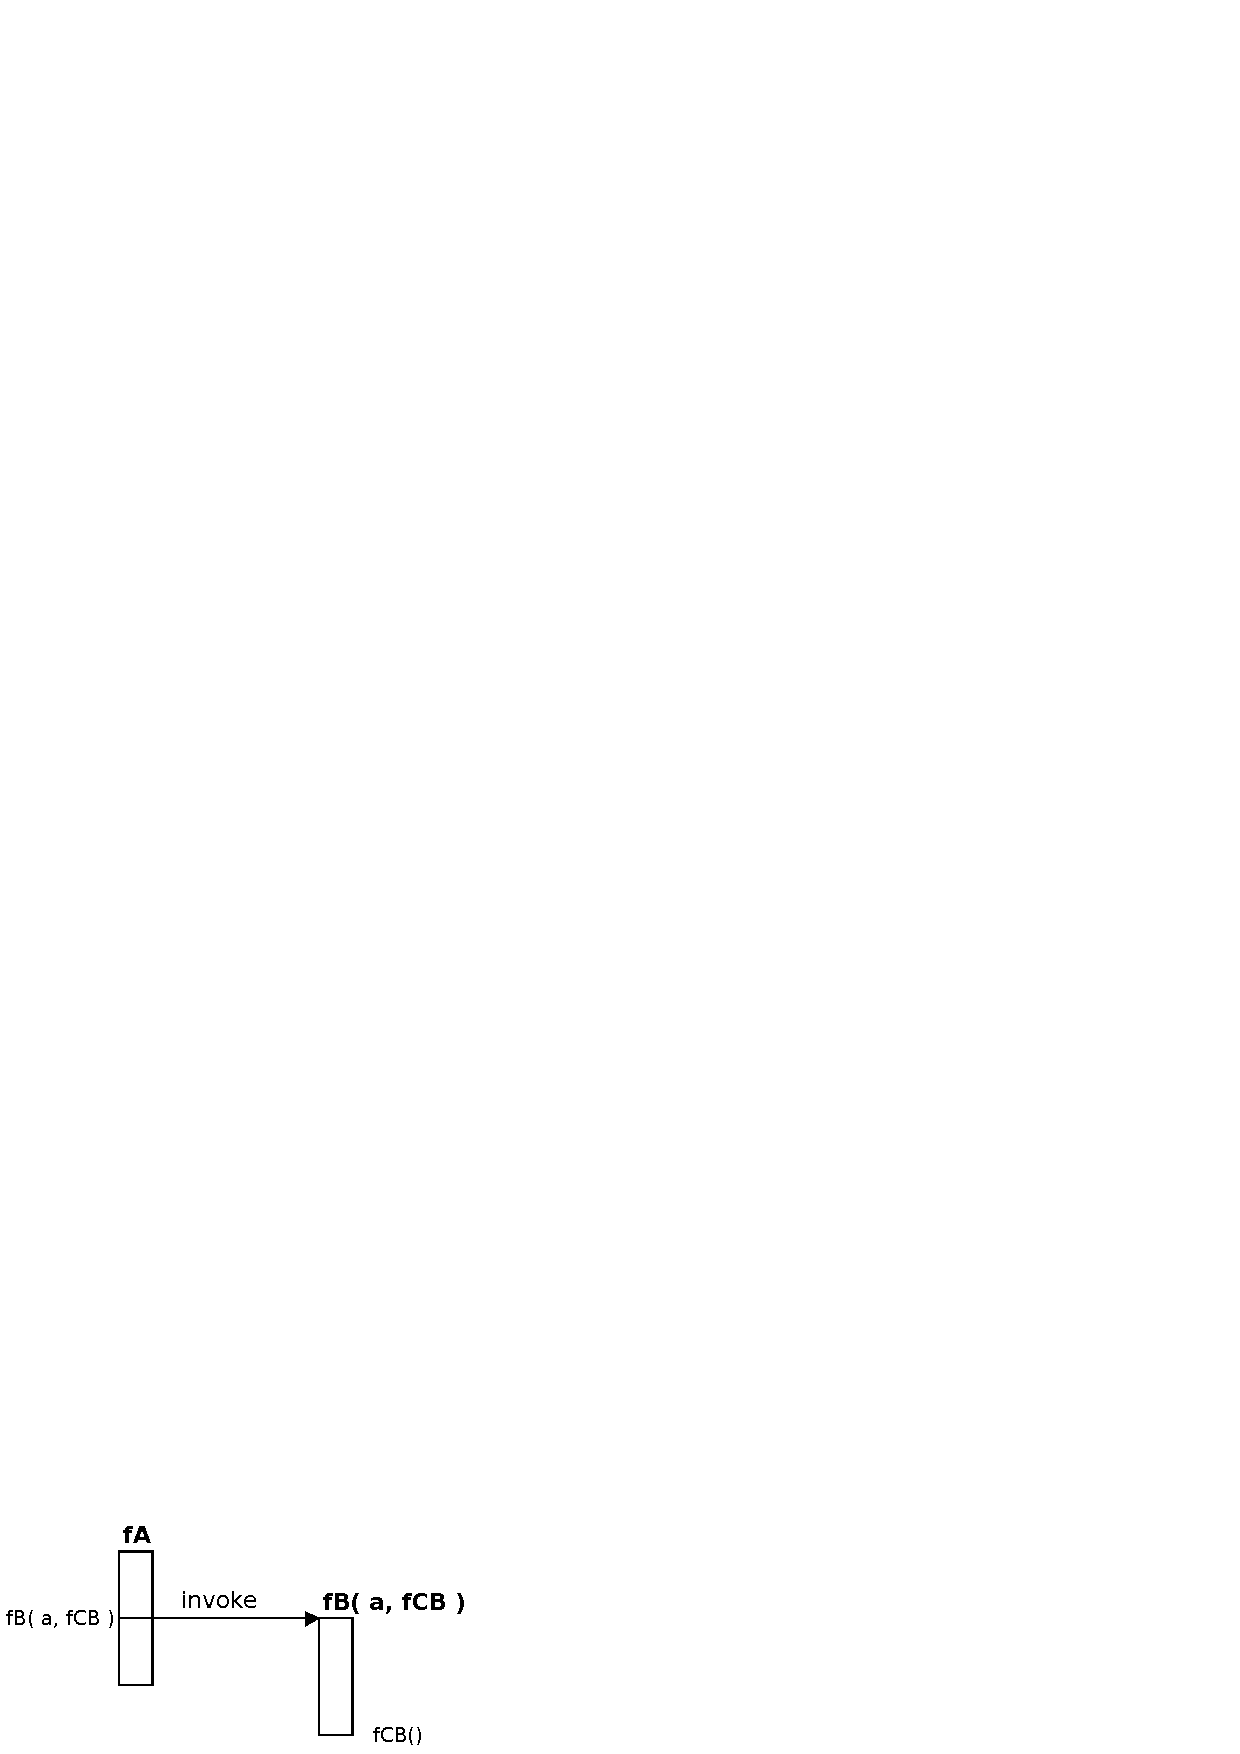
\includegraphics{figures/Closures_Asynchronous}
\caption{Asynchronous Function Call}
\label{fig:Closures_Asynchronous}
\end{figure}


Often other operations depend on the completion of asynchronous operations, hence their execution needs to be deferred.
This necessary code execution deferral is achieved through the use of callback functions, denoted \texttt{fCB} in figure~\ref{fig:Closures_Asynchronous}.
Any code placed in a callback function, which is assigned to an asynchronous operation, is only executed after the respective asynchronous operation completed.
This allows stacking of functions and operations upon each other which results in a flexible, event driven application.


If we look at the example in figure~\ref{fig:Closures_Asynchronous} and assume closures as defined in \cite{EcmaScript}, .
 


\begin{figure*}[htb]
%\begin{center}
\centering
%,angle=-90
  \makebox[\textwidth][c]{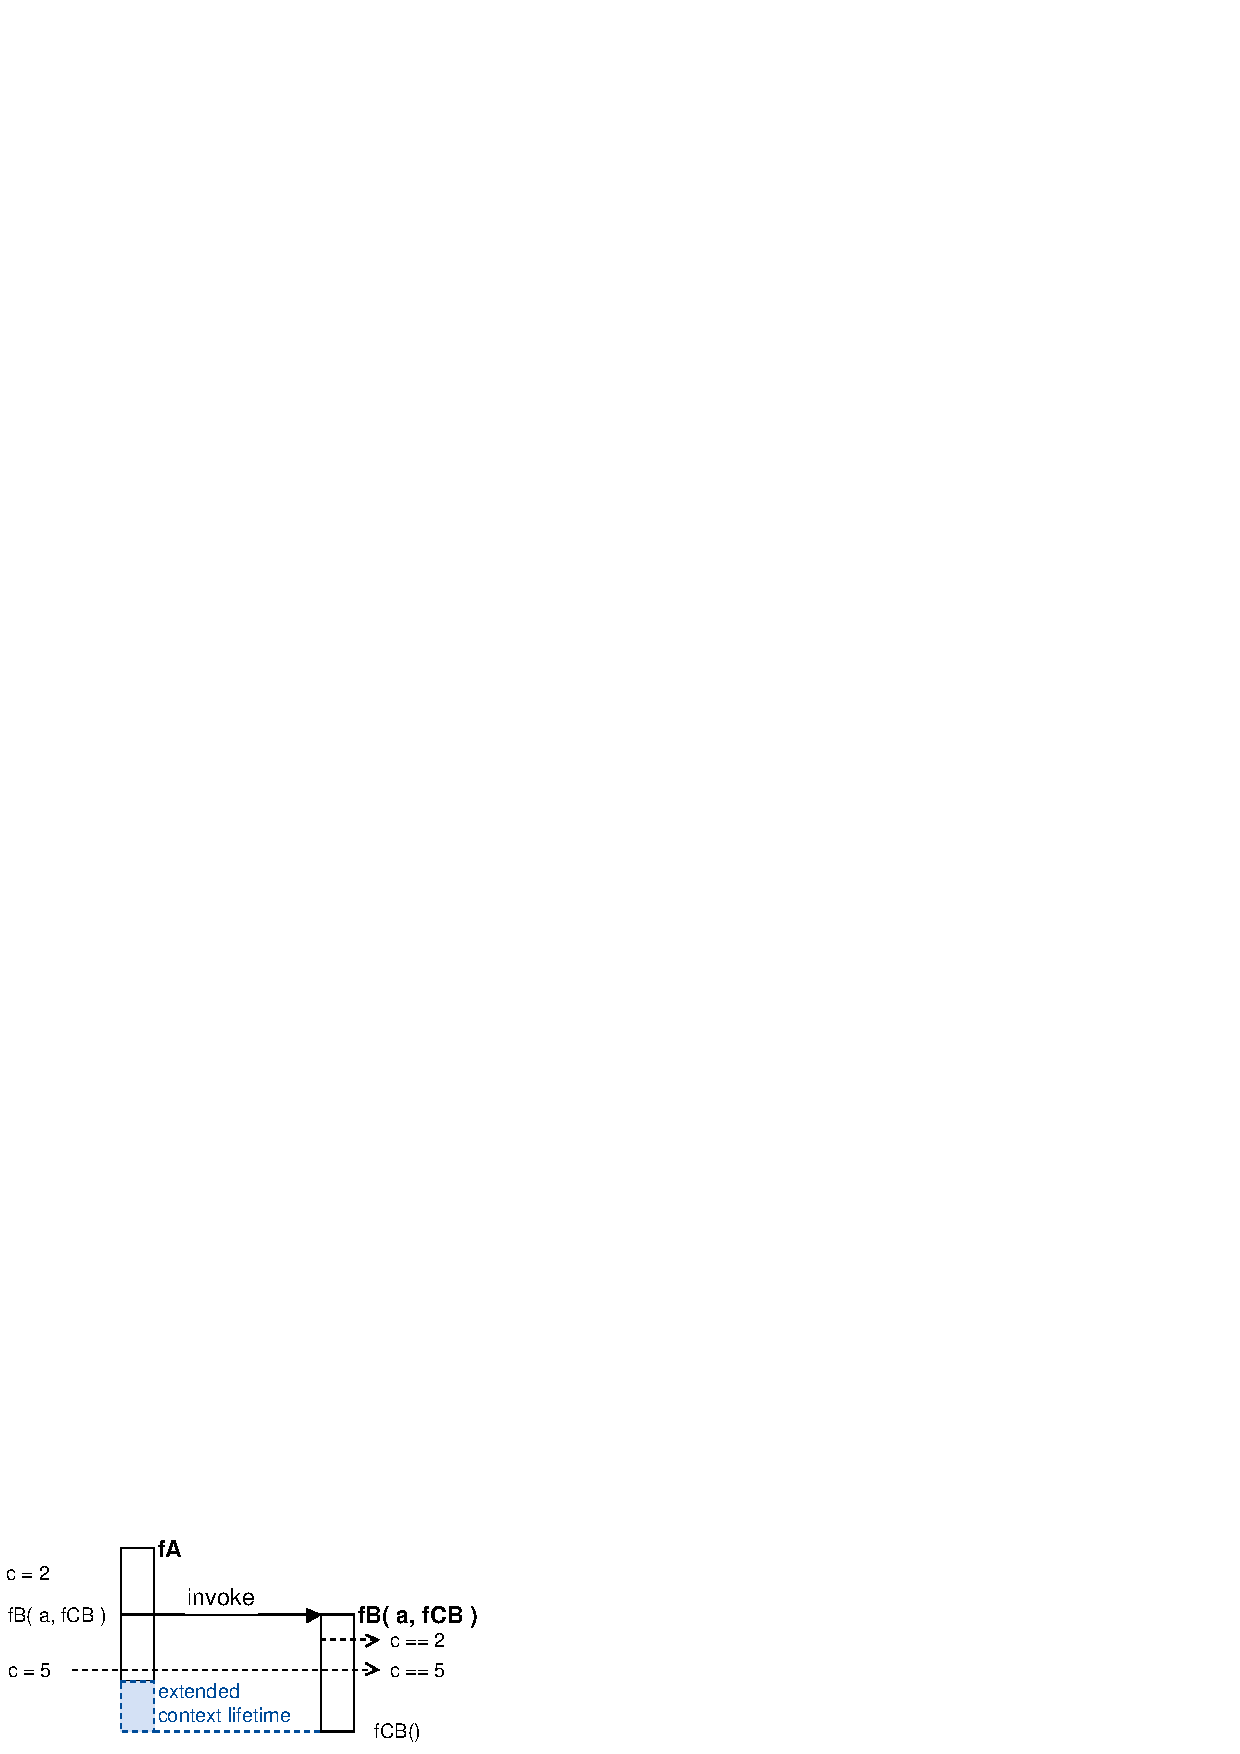
\includegraphics{figures/Closures_Closure-1}}%
\caption{Closure Scope}
%\end{center}
\end{figure*}


\begin{figure*}[htb]
%\begin{center}
\centering
%,angle=-90
  \makebox[\textwidth][c]{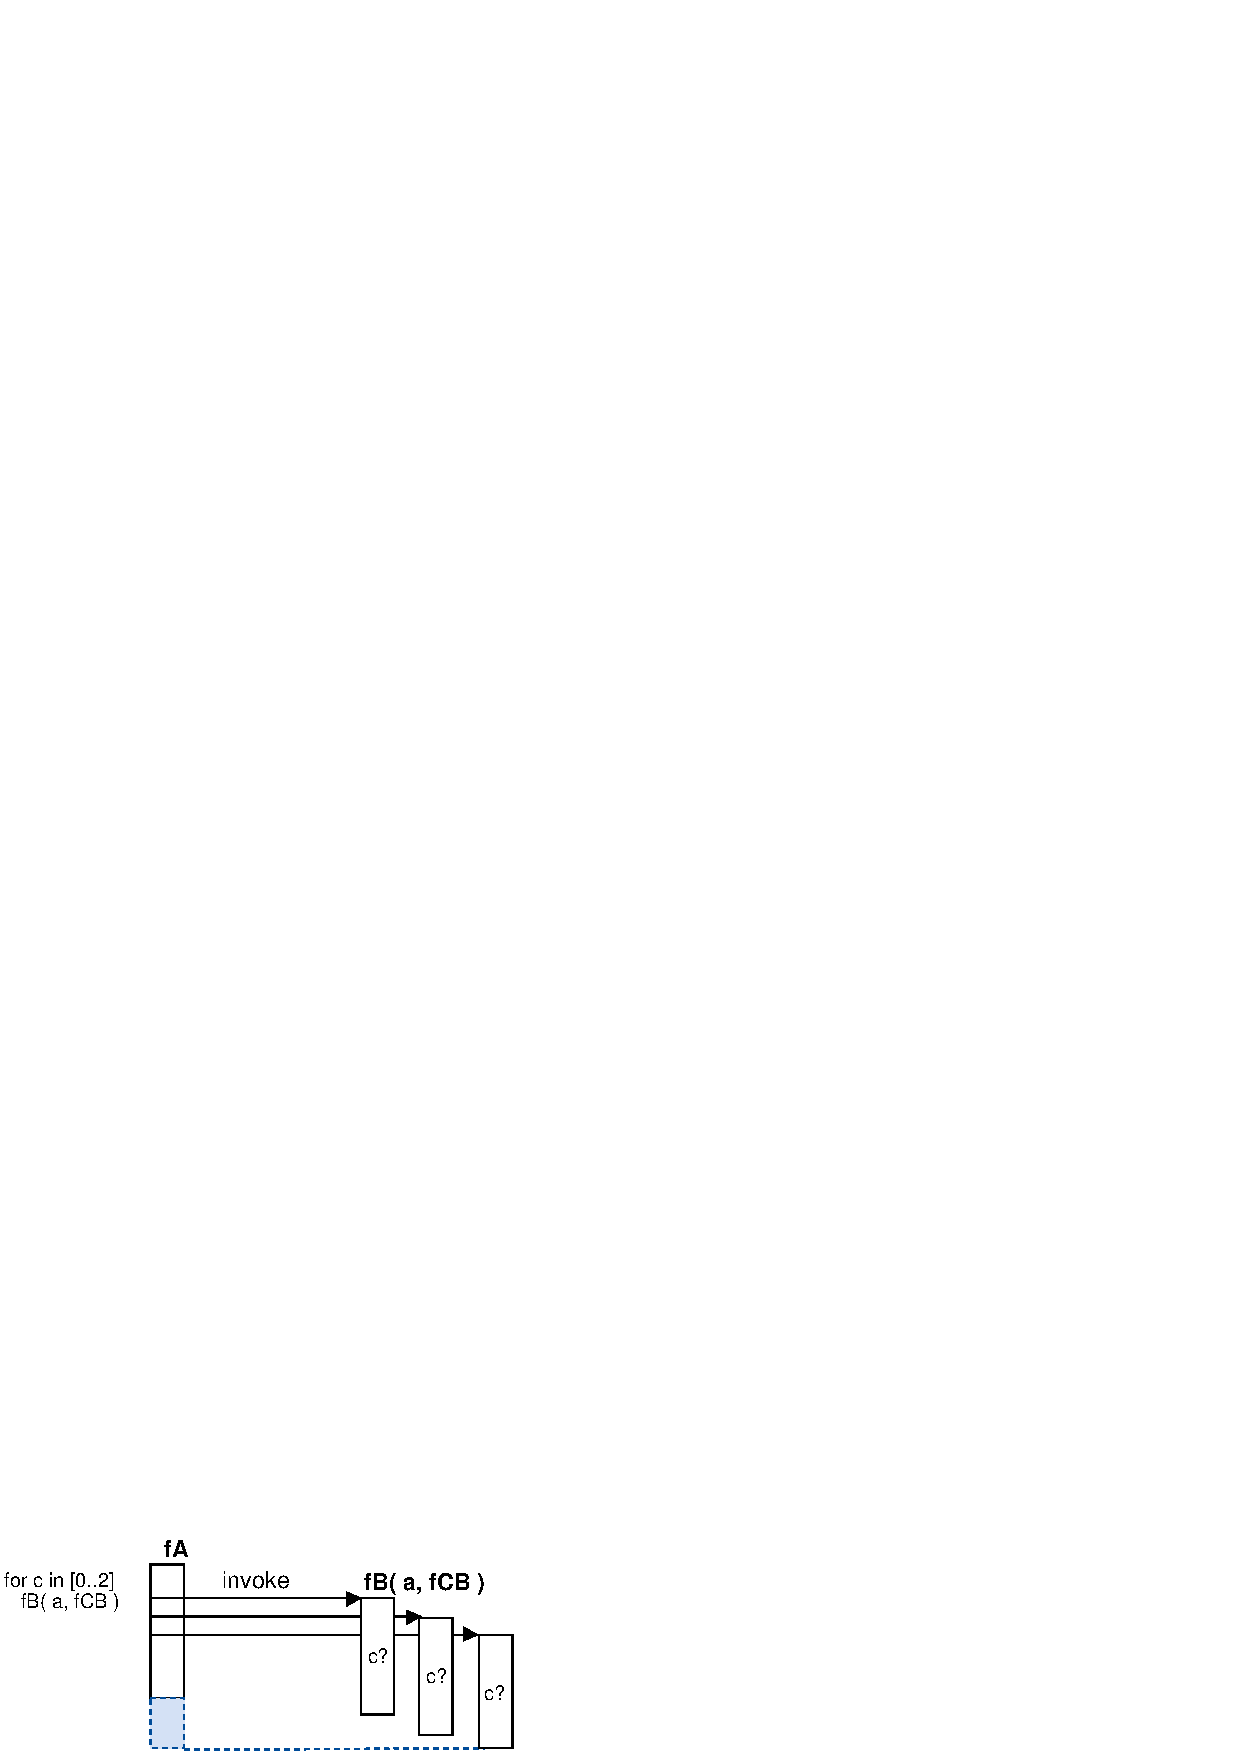
\includegraphics{figures/Closures_Closure-2}}%
\caption{Closure Scope}
%\end{center}
\end{figure*}


\begin{figure*}[htb]
%\begin{center}
\centering
%,angle=-90
  \makebox[\textwidth][c]{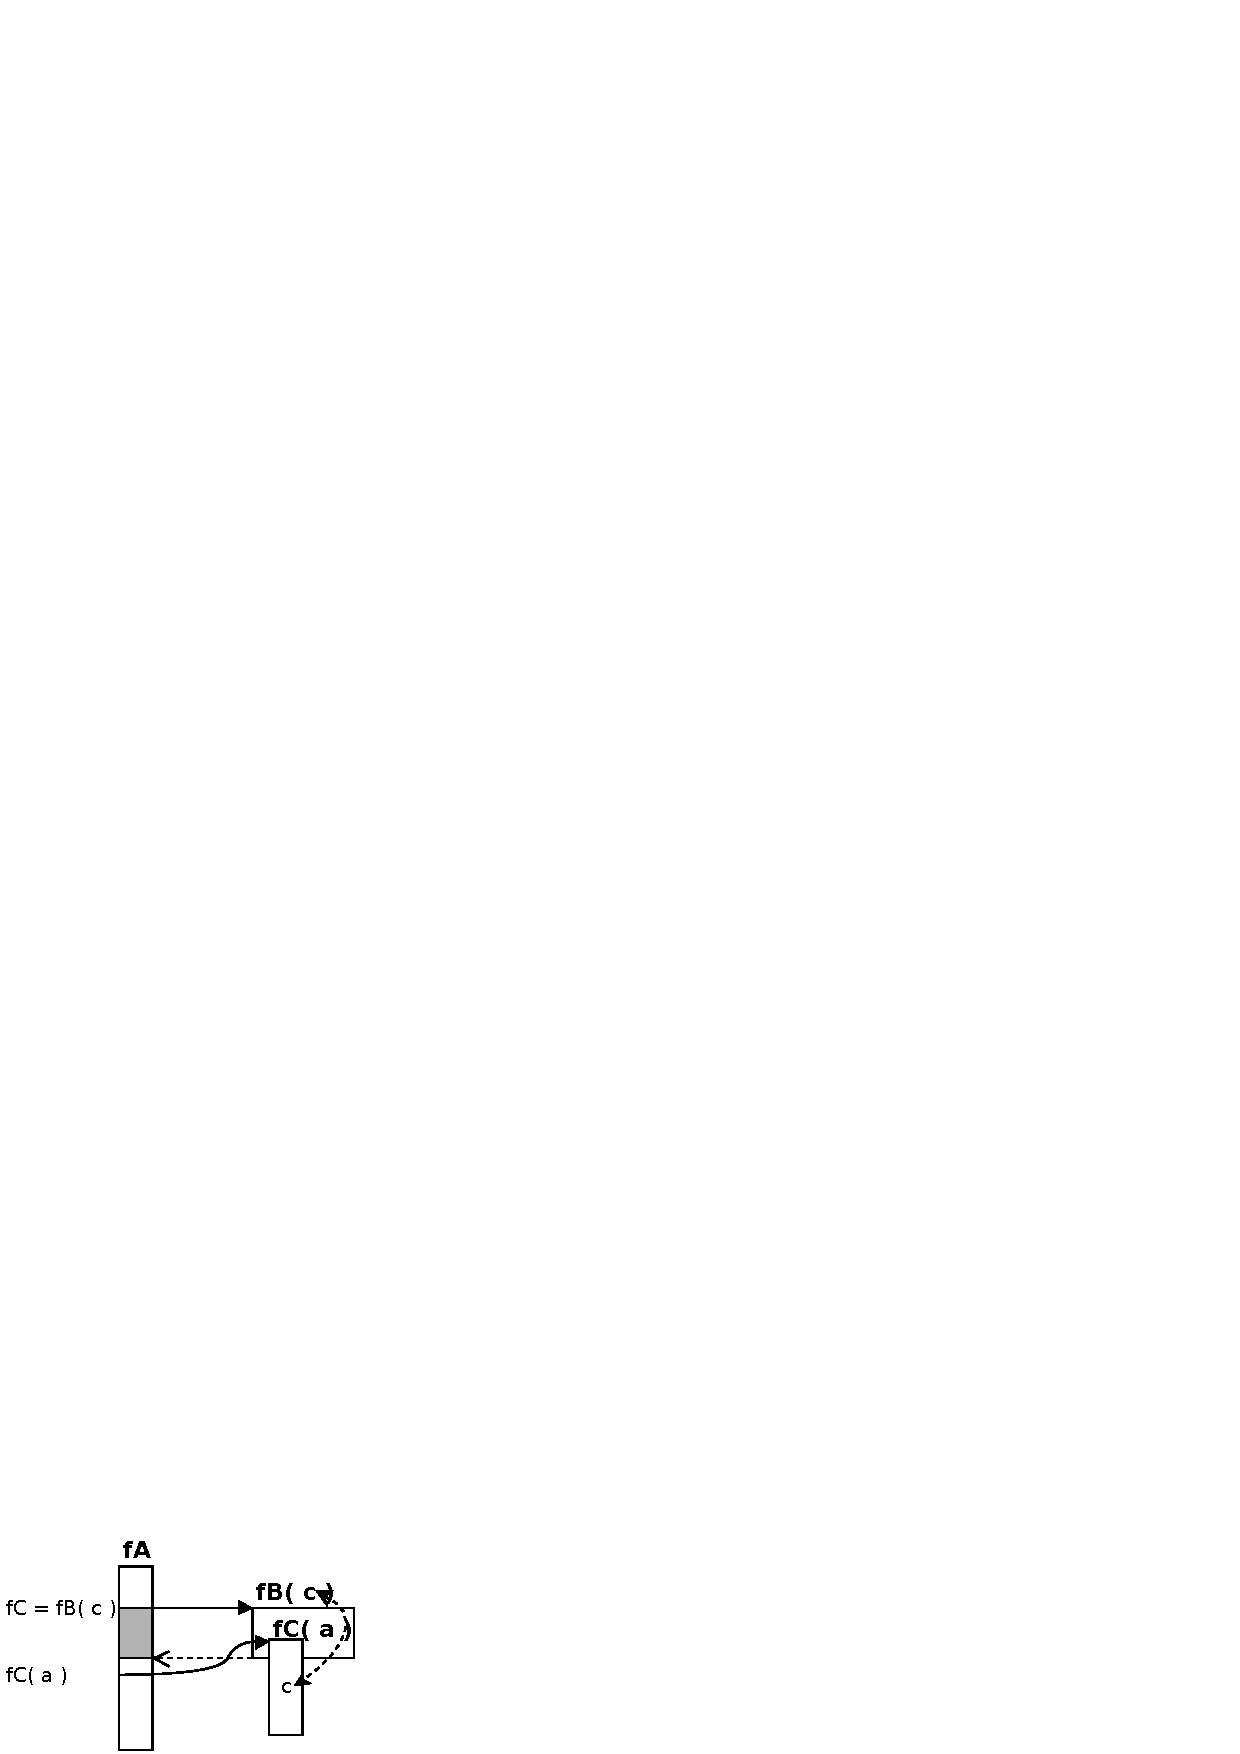
\includegraphics{figures/Closures_Closure-3}}%
\caption{Closure Scope}
%\end{center}
\end{figure*}

% Error tracing
% Apply variable number of function arguments to function

	
\chapter{Discussion \& Results}



\subsection{Use Cases}
% NOTES / TODOs:
%
% Temperature warning, using import.io
% Tutorial example: as seen by user, as seen by the developer
%http://khanlou.com/2014/03/model-view-whatever/

\newpage


\section{Future Work}
% NOTES / TODOs:
%
% CEP
We have seen that the ECA approach is already a powerful one to make the web reactive.
A future improvement of this could be to adopt Complex Event Processing (CEP).
This would mean that several events could be stored in a rule and be evaluated in terms of time constraints.
Through this more complex events can be created as a result of several atomic events which would lead into semantically more complex events.
A change in paradigm will result in an approach where events are not just processed when they are entering the system and evaluated against rules, but these events would need to be stored for quite a long time.
Also the rules will not all be checked for each event but they are subject to a scheduler.
It can be decided when and how often a rule is evaluated and all events will be checked at these point in times, whether they are candidates for firing the rule.
A relational database will be needed in order to search through the timestamps
\backmatter
	\begin{Verbatim}[fontsize=\small,commandchars=\\\{\}]
\PY{l+s}{\PYZsq{}}\PY{l+s}{use strict}\PY{l+s}{\PYZsq{}}\PY{p}{;}
\PY{n}{var} \PY{n}{express} \PY{o}{=} \PY{n}{require}\PY{p}{(}\PY{l+s}{\PYZsq{}}\PY{l+s}{express}\PY{l+s}{\PYZsq{}}\PY{p}{)}\PY{p}{;}
\PY{n}{var} \PY{n}{qs} \PY{o}{=} \PY{n}{require}\PY{p}{(}\PY{l+s}{\PYZsq{}}\PY{l+s}{querystring}\PY{l+s}{\PYZsq{}}\PY{p}{)}\PY{p}{;}
\PY{n}{var} \PY{n}{engine} \PY{o}{=} \PY{n}{require}\PY{p}{(}\PY{l+s}{\PYZsq{}}\PY{l+s}{./ecainference}\PY{l+s}{\PYZsq{}}\PY{p}{)}\PY{p}{;}
\end{Verbatim}
	\addcontentsline{toc}{chapter}{Bibliography}
	\bibliography{thesisbib}
	\bibliographystyle{thesisbst}
	\listoffigures
	\listoftables
	\lstlistoflistings
	\addcontentsline{toc}{chapter}{Index}
	\printindex
\end{document}
